\documentclass[]{rsos}%%%%where rsos is the template name

%%%% *** Do not adjust lengths that control margins, column widths, etc. ***


%%%%%%%%%%% Defining Enunciations  %%%%%%%%%%%
\newtheorem{theorem}{\bf Theorem}[section]
\newtheorem{condition}{\bf Condition}[section]
\newtheorem{corollary}{\bf Corollary}[section]
%%%%%%%%%%%%%%%%%%%%%%%%%%%%%%%%%%%%%%%%%%%%%%%



\begin{document}

%%%% Article title to be placed here
\title{Survival depends critically on predator detection in zebrafish larvae}

\author{%%%% Author details
Arjun Nair, Christy Nguyen, and Matthew J. McHenry}

%%%%%%%%% Insert author address here
\address{Department of Ecology and Evolutionary Biology\\
University of California, Irvine\\
321 Steinhaus Hall\\
Irvine, CA 92697}

%%%% Subject entries to be placed here %%%%
\subject{Animal behavior, biomechanics}

%%%% Keyword entries to be placed here %%%%
\keywords{Game theory, locomotion, predation, sensing, strategy}

%%%% Insert corresponding author and its email address}
\corres{Matthew J. McHenry\\
\email{mmchenry@uci.edu}}



%%%%%%%%%%%%%%% End of first page %%%%%%%%%%%%%%%%%%%%%

\maketitle

%%%%%%%%%% Insert the texts which can accomdate on firstpage in the tag "fmtext" %%%%%

%\begin{fmtext}


\linespread{1.6}\selectfont %Doublespacing


\section*{Abstract}
Predation is a fundamental interaction between animals, yet it is largely unclear how prey survive encounters with predators.
Using experiments and game modeling, we examined the relative contributions of sensing and locomotion to larval zebrafish when they escape older fish of the same species.
High-speed 3D kinematic measurements of interactions between an individual prey when encountering a predator were used to establish the probability distributions of behavioral parameters for both fish.
These measurements provided the basis for a game model that predicted the trajectories of predator and prey. 
Upon verifying that the model could replicate the frequency distribution of the number of strikes that prey survived, we conducted a sensitivity analysis to determine which parameters had the greatest influence on prey survival.
This analysis found that escape direction and the predator's speed and strike distance has negligible effects on prey survival.
Survival instead depends on the reaction distance and escape speed of prey. 
For example, \hl{prey are half as likely to survive if they respond at half the distance of what was observed experimentally}.
\todo[fancyline]{True? I guessed this by looking at the graph.}
A comparable effect may be achieved with a more extreme reduction in escape speed. 
Therefore, strategy in piscivorous interactions depends critically on the ability of prey to detect predators at a distance.
This finding informs our understanding for the sensory ecology of a broad diversity of fishes and may indicate a general dynamic in predator-prey interactions.


\section{Introduction}

Predator-prey interactions offer a context for understanding the biomechanics and neurophysiology of animals.
It is commonly argued that the survival of evasive prey and the success of predators depend on fast or highly maneuverable locomotion \cite{Alexander:BbR35qCj, Wilson:2013fda, Walker:2005vn}.
The rate and force of predatory strikes are similarly considered important factors \cite{deVries:2012tc, Holzman:2009uu}, as is the ability of prey to sense an approaching predator at great distance \cite{Dill:1972wh, Gabbiani:1999wz}.
However, it is not clear how these factors compare in their strategic importance to prey survival and it is consequently unknown what traits distinguish successful predators and prey. 
The aim of the present study was to determine the variables that are most important in determining the survival of a fish when it becomes the prey of a larger fish.

Understanding the dynamics of predators and prey is challenged by the interdependency of both animal's actions.
Any motion by a prey may (or may not) be in response to the predator, which may (or may not) be a response to an earlier motion by the prey. 
This behavioral coupling has the potential to make the behavior of predator or prey appear as a stochastic chain of events.
Multivariate statistics are generally insensitive to such dynamics, yet may resolve exceptional features of successful prey \cite{Walker:2005vn} or predators \cite{Wainwright:2001ufa}.
Such analysis is enhanced by considering behavioral responses to an artificial predator or prey that is experimentally controlled \cite{Gabbiani:1999wz,Stewart:2014cma}.
An alternative approach explicitly considers the kinematics of one agent in an attempt to resolve the strategy of the other.
For example, bat predators have been shown to track evasive moths by maintaining their heading, rather than attempting to anticipate the prey's direction \cite{Ghose:2006dk}. 
This finding was resolved by comparing the measured trajectory of predators to that predicted by a behavioral algorithm, given the measured motion of prey.

The strategic implications of predator and prey behavior have been considered through applications of game theory.
This area has capitalized on the development of mathematical modeling in two areas.
Biologists concerned with Search games 


Such agent-based modeling 
Predator-prey strategy may alternatively be considered with game theory.

Game theory offers an analytical toolkit for studying the strategic implications of locomotion and sensing . . .
\hl{cite Weihs' paper, Alberto's paper, Casas...}
Differential game theory, as it has been applied to predator-prey interactions, is purely deterministic and consequently offers the opportunity to resolve optimal strategies by analytical mathematics. . .

The present study addressed the strategic importance of sensing and locomotion using a combination of experiments and mathematical modeling. 
High-speed kinematics were recorded for the swimming by individual zebrafish larvae as they were pursued by individual adult predators of the same species, as in previous studies \cite{Stewart:2014cma, Soto:2015cj}.
Descriptive statistics of these interactions were used to characterize the probability of behavioral actions by both the predator and prey.
These findings provided the basis of a game model that was used to simulate the conditions of our experiments. 
Once verified, an analysis of this model was performed to evaluate the sensitivity of prey survival on the behavioral parameters of the predator and prey.


\section{Material and methods}

\subsection{Animal husbandry}
All experiments were conducted on zebrafish (\textit{Danio rerio}, Hamilton 1922), where larvae (5 -- 7 days post fertilization, dpf) were preyed upon by older fish of the same species. 
To examine how these interactions vary with the size of the predator, we performed one set of experiments using adult ($\geq 9$ months old, $\SI{3.4}{\cm} \pm \SI{0.5}{\cm}$) predators and another using juveniles ($3-4$ months old, $\SI{2.0}{\cm}  \pm  \SI{0.4}{\cm}$). 
Although similar in shape, adults were significantly larger in body length and gape diameter than juveniles (adults: \hl{$\SI{0.240}{\m} \pm \SI{.0004398}{\m}$, juveniles: $\SI{0.238}{\m} \pm \SI{.0003058}{\m}$}
\todo[fancyline]{24 cm in length?!  You mean 2.4 cm, I presume?  Also, the SD should not have greater decimal places of preceision than your mean.  I would go with "cm" instead of "m" for units}
, One-way ANOVA, $N = 19$).
All fish were bred from wild-type (AB line) colonies housed in a flow-through tank system (Aquatic Habitats, Apopka, FL, USA) that was maintained at $\SI{28.5}{\celsius}$ on a 14:10 h light:dark cycle. 
To produce larvae, the fertilized eggs from randomized mating were cultured according to standard techniques \cite{Westerfield:UXiBrEuA}.
Predators were motivated to feed by fasting for a period of 7 -- 14 days prior to an experiment.


\subsection{Kinematics}
We arranged the lights and cameras for high-speed recordings of both fish with high-contrast images. 
A hemispherical aquarium ($\oslash = \SI{8.5}{\cm}$) was composed of white acrylic, which served as a translucent diffuser of the IR illumination (940 nm) provided by three lamps (CM-IR200-940, CMVision, Houston, TX, USA), positioned below (Fig. \ref{fig_setup}a). 
These lamps provided high-intensity illumination that was invisible to the fish (\hl{CITE})
\todo[fancyline]{You might as well resolve all citations you know we're going to need}
, while visible illumination at low intensity was provided by overhead fluorescent lights.
Each camera (FASTCAM Mini UX50, Precision Photron Inc., San Diego, CA, USA) was fitted with a with a 55mm lens (f/2.8 Micro Nikkor AIS, Nikon Inc., Melville, NY, USA) and positioned at a distance to permit a view of the entire aquarium. 
The cameras were arranged above the aquarium to allow both fish to be viewed by at least two cameras when the fish were positioned close together.
The cameras were synchronized to record at 1,000 fps (at \hl{1024}
\todo[fancyline]{not 1280? That's what the sensor does, but maybe you cropped it with the software?}
 x 1024 pixels) with a common TTL end-trigger and controlled with the manufacturer's software (PhotronFASTCAM Viewer).

Predation experiments were performed by recording the swimming of one predator and one prey fish in the aquarium (Fig. 1A). 
This began by placing the fish on opposite sides of a partition.
Following a 15 min acclimation period, we lifted the partition and observed the fish until the predator successfully ingested the prey.
Using a post-trigger to the high-speed cameras, we saved recordings from $\sim \SI{0.5}{\s}$ before the first predatory strike and until $\sim \SI{0.5}{\s}$  after the prey was captured.

Our video recordings were used to perform measurements of 3D kinematics. 
We calibrated the cameras by recording a static body that we constructed with 48 landmarks of known relative position, which was placed in the center of the aquarium.
A direct-linear transform (DLT) was calculated using `Digitizing Tools' software in MATLAB (2015a, MathWorks, Natick, MA, USA) \cite{Hedrick:2008wz} from manually-selected coordinates of these landmarks from the perspective of the three cameras.
Using a custom script in MATLAB, we found the body positions of predator and prey fish by selecting landmarks from two camera views and using the DLT to determine the coordinates in 3D space.
We used the position of the predator's two eyes to calculate a mean position that approximated the buccal cavity (Fig. \ref{fig_setup}a).
The rostrum and posterior margin of the swim bladder were found on the prey's body. 
The posterior of the swim bladder approximates the center of mass \cite{Stewart:2010ig}.
We acquired the landmark positions at five key events in each interaction between predator and prey: (1) when the predator initiated an approach toward the prey, when the predator (2) began and (3) completed suction feeding and (4) at the initiation and (5) completion of the prey's escape response.


\subsection{Descriptive statistics}

Descriptive statistics were used to characterize the probability of actions by the predator and prey during predation experiments.
For all interactions recorded among our experiments, we found predator-specific parameters that consisted of the strike distance ($s$), the distance from the prey at which a strike was initiated, and the strike duration ($\tau$), which is the period between the opening and closing of the mouth during suction feeding. 
For the prey, we found the reaction distance ($l$), which is the distance from the predator at which the escape response is initiated.
The escape was additionally characterized by the escape angle ($\theta$), the angular change in heading from the resting orientation to the escape path.
The escape duration ($\eta$) included the period for all stages of the C-start and subsequent undulatory swimming, until the larva ceased motion.
The frequency distribution for each parameter was found to be well-approximated by the following log-normal probability density function:
%
\begin{equation}%%% Equation lognormal distribution
f(x) = \frac{1}{x\sigma \sqrt{2 \pi}} \text{exp} \left[ -{\frac{(ln(x)-\mu)^2}{2\sigma ^2}} \right],
\label{eqn_lognorm}
\end{equation}
%
where $x$ is a particular behavioral parameter ($s, \tau, l, \theta ,$ or $\eta$), $\mu$ is the log mean, and $\sigma$ is the log standard deviation. 
We determined best-fit values for $\mu$ and $\sigma$ for each behavioral parameter by maximum-likelihood (the `fitdist' function in MATLAB).

The probability that the strike of a zebrafish predator is successful depends critically on the distance between the mouth and the prey \cite{Stewart:2013bha}.
Strikes were therefore measured as a function of distance. 
These measurements revealed that the probability of a successful capture $(C)$ was well-characterized by the following sigmoidal function:
%
\begin{equation}%%%Equation for sigmoid function
C(d) = \left[ 1+e^{-r(d-d_0)} \right]^{-1},
\label{eqn_sig} 
\end{equation}
%
where $d$ is the distance between predator and prey, $d_0$ is the decay distance, and $r$ is the decay rate. 
The best-fit values for $d_0$ and $r$ were determined by least-squares (`sqcurvefit' function in MATLAB).

All parameters for the prey and predators were compared between experiments with adult predators and juvenile predators.
These parameters failed to conform to normal distributions, so we performed comparisons with non-parametric statistics. 
In particular, probability-density functions (Eqn. \ref{eqn_lognorm}) and capture probability (Eqn. \ref{eqn_sig}) parameters were compared using a two-sample Kolmogorov-Smirnov test (i.e. KS-test) (\hl{CITE}). 
\todo[fancyline]{Might as well do this now}

\subsection{Game model}
\todo[inline]{I've changed my mind (again): I think the model can be described better in the past tense.}

A pursuit-evasion game model was developed to simulate the conditions of our experiments. 
This model predicted the 2D motion of a predator (i.e. pursuer) and prey (i.e. evader) according to algorithms that were specific to the behavioral state of each of these agents (Fig. \ref{fig_setup}b). 
The predator's states were Tracking (T) and Striking (S) and the prey's were Resting (R) and Escaping (E). 
The duration of states, probability of transitioning between states, and probability of capture were determined by random-number generators with probability distributions and a range of values that matched the results of our kinematic measurements.
Therefore, the model treated the predator and prey's actions as probabilistic, but each outcome of an interaction also depended on the determinism of the kinematics of the two agents.
Simulations were scripted in MATLAB to calculate the motion of both agents and their behavioral states and consequently determined the number of unsuccessful strikes before prey capture.

Each simulation began with the predator in the Tracking state, where it moved at an approach speed $U$ with a direction that was always headed toward the prey, with perfect information about the prey's position (Fig. \ref{fig_setup}b). 
If the prey was motionless, then the solver would advance in time to the strike or escape initiation, whichever was found to occur first.
Otherwise, the predator tracked the motion of the prey with a delay, $\lambda$, calculated with a fixed time step of \SI{5}{\ms}.  
The predator's transition into the Striking state was determined when the prey was within a particular value for strike distance ($s$). 
This value was determined \textit{a-priori} by the generation of a random value (using the `random' function in MATLAB) from the log-normal probability-density function (Eqn. \ref{eqn_lognorm}) for measured values of $s$.
The capture probability for a particular strike depended on the distance between the agents in the middle of a strike, according to our measured parameter values for this relationship (Eqn. \ref{eqn_sig}).
Our simulations used this relationship to generate a random value for the range within which the prey was determined to be captured.
The simulation was terminated if a strike was successful, otherwise the predator reverted to the Tracking state after completion of the strike duration.
Single values for the approach speed and predator delay were used for all simulations (Table \ref{table}) and were determined by trial-and-error to best replicate the distribution of the measured number of unsuccessful strikes before prey capture. 
These values approximated measurements reported in prior studies \cite{McHenry:2005tc, Stewart:2013bha}. 

The game model simultaneously determined the actions of prey (Fig. \ref{fig_setup}b).
Prey behavior was modeled with Resting and Escaping states because larval zebrafish generally remain still between periods of rapid swimming initiated by an escape response \cite{Stewart:2013bha, Stewart:2014cma}. 
The prey began each simulation in the Resting state, where it was motionless at a random distance equal to, or less than, the aquarium diameter ($\oslash = \SI{8.5}{\cm}$) and at a random orientation with respect to the predator.
The prey transitioned into the Escaping state when the predator moved within the reaction distance ($l$) after a latency ($\chi$) \cite{Nair:2015gk}.
During an escape, the prey was assumed to follow a straight path in the direction of the escape angle ($\theta$).
Using a frame-by-frame kinematic analysis of escape swimming for 12 larvae, we found that prey varied speed as a saw-toothed function of time that approximately attained its maximum value at 20\% of the duration duration. 
We consequently modeled variation in swimming speed for prey to attain the maximum speed ($u$) was achieved at 0.2$\eta$, where $\eta$ is the escape duration. 
The reaction distance, escape angle, and escape duration were determined by random numbers with probability density functions matching experimental measurements.
The escape angle was defined with respect to the prey's frame of reference, with $\theta =  \SI{0}{\degree}$ corresponding to forward motion.
The escape direction ($\upsilon$) was defined as the probability that this angle was directed away from the predator, with a value (Table \ref{table}) that was previously measured \cite{Stewart:2014cma}.

This model simplified many aspects of the complexity of predator-prey interactions.
It assumed that the kinematics of the two fish may be reasonably approximated with two-dimensional motion that is not bounded by an aquarium. 
Simulations were stopped if prey successfully escaped on 20 occasions, which reflected the observed maximum and guarded against an errant simulation of infinite duration.
The model's probabilistic approach considered the effects of biomechanics and neurophysiology without articulating those elements.
For example, capture success was treated as a distance-specific probability (Eqn. \ref{eqn_sig}) that parsed neither the effects of a predator's suction-feeding hydrodynamics, nor the propulsive forces generated by an escaping prey.
The number of successful escapes before capture for all experiments were compared to the same metric for 1,000 simulations.  
This comparison was executed by a two-sample Kolmogorov-Smirnov test, chosen over a Kruskal-Wallis test because of its emphasis on the shape of the distribution.  

A sensitivity analysis evaluated the characteristics of the predator and prey behavior which had the greatest effect on prey survival. 
This was achieved by running batches of a 1,000 simulations with parameters varied individually between -90\% and 100\% of their original mean values at increments of 10\%.
For parameters described by a probability distribution, the log-mean $\mu$ parameter and the range of values were adjusted to create the desired percent-change in the mean of the distribution.
The effect of these manipulations were assessed by comparing the measured escape probability against the model's prediction using a Kruskal-Wallis test. 



\section{Results} %==================================================================

\subsection{Kinematics} %==========
The behavior of both predator and prey were similar whether the predators were juvenile or adult zebrafish.
Prey responded with similar behavior, having indistinguishable differences in escape angle (KS-test: $P = 0.86, N = 164$) and with modest, though significant, differences in reaction distance (KS-test: $P < 0.001, N = 164$) and escape duration (KS-test: $P = 0.04, N = 153$) (Fig. \ref{fig_PDF}\textit{b--c}). 
For example, prey responded at a mean distance to juvenile predators ($\overline{l} = \SI{8.4}{\mm}, N = 91$), at about two-thirds the reaction distance to adults ($\overline{l} = \SI{12.6}{\mm}, N = 73$).
Escape swimming lasted for about one-third of a second, with the response to juveniles ($\overline{\eta} = \SI{0.35}{\s}$, $N$ = 91) being only  $\SI{50}{\ms}$ longer than to adults ($\overline{\eta} = \SI{0.30}{\s}$, $N$ = 62).
Juvenile and adult predators were significantly different in neither their strike distance (KS-test: $P = 0.08, \overline{s} = \SI{7.6}{\mm}, N = 154$), nor strike duration (KS-test: $P = 0.87, \overline{\tau} = \SI{44}{\ms}, N = 107$) (Fig. \ref{fig_PDF}\textit{d--e}).
Therefore, much of the behavior of predator and prey were similar, despite the fact that the adults were nearly twice the body length of the juveniles.

The major exception in this comparison was in the effectiveness of strikes by suction feeding.
Juveniles did not succeed in capturing prey beyond a distance of $\SI{3.2}{\mm}$ ($N = 91$), whereas adults captured prey at a maximum distance that was 3-times greater ($\SI{10.4}{\mm}, N = 77$).
In the relationship between capture probability and distance (Eqn. \ref{eqn_sig}), the decay distance indicates the spatial range of high capture probability. 
By this metric, the strike of adult predators also exhibited a range that was slightly greater than 3-times the distance of juveniles (Table \ref{table}, Fig. \ref{fig_PDF}\textit{f}).
Therefore, the spatial proximity of suction feeding is the key feature that distinguishes the performance of juvenile and adult predators.

\subsection{Game model} %==========
The trajectories of predator and prey fish followed paths that were qualitatively similar to that predicted by our game model.
For most of the duration of our experiments, predators were observed to be swimming toward the prey (Fig. \ref{fig_traj}a). 
In contrast, the prey were generally motionless, unless interrupted by undulatory swimming, initiated with a fast-start.
The predators and prey followed a more circuitous path toward to prey than the motion prescribed by our model (Fig. \ref{fig_traj}b).
Nevertheless, the temporal sequence of events in the model offered a reasonable approximation of the kinematics of live predator-prey interactions.

The model accurately predicted the broad quantitative patterns of our experimental results.
This was assessed by the probability of the prey surviving over a particular number of strikes. 
In our experiments, prey exhibited the greatest probability of being captured on the first strike with monotonically lesser probabilities over subsequent strikes (Fig. \ref{fig_traj}c).
Adults were more successful on the first, second and third strikes than the juveniles, which consequently exhibited a more even probability distribution.
The model was successful in replicating these trends, which were found to be statistically indistinguishable for both adult (KS-test: $P = 0.93, N = 73$) and juvenile (KS-test: $P = 0.86, N = 91$) predators. 
Furthermore, \hl{all trends from the game model were similar between the juvenile and adult predators. Therefore, adult game model results are presented in this results section and juvenile predator results from the game model are presented in the supplemental material}\todo{what's this in reference to? Sensitivity analysis? Be specific.}(Fig. \hl{Supp. Mat.}).


A sensitivity analysis of prey parameters revealed that escape speed and reaction distance were the only parameters with a substantial effect on prey survival. 
Changes in escape duration, escape direction, and escape angle led to statistically insignificant or small changes in escape probability (Fig. \ref{fig_sense}a). 
On contrast, \hl{modulating reaction distance and escape speed changed the escape probability, on average, by 23\% and 15\%,}\todo{not sure what this means} respectively, over the other three \hl{parameter modulations}\todo{?}.
By increasing the mean value of the reaction distance, escape probability increased significantly by upwards of 16\%. 
However, decreasing the mean value of the reaction distance created greater, significant decreases to the escape probability, \hl{as great as 70\%}\todo{over how much reduction in distance?}. 
Increasing escape speed did not lead to a significant increase in escape probability and significant decreases to escape probability only occurred when escape speed was reduced by 50\% or more of its original value.

We examined whether escape speed and reaction distance interactively affect escape probability by conducting a two-dimensional sensitivity analysis (Fig. \ref{fig_sense}\textit{b}).
This yielded results which were consistent with our initial analysis (Fig. \ref{fig_sense}\textit{a}). 
For a particular escape speed, increasing reaction distance above the measured value slightly, though significantly, increased the overall escape probability. 
However, a decrease in reaction distance generated large decreases in escape probability (Fig. \ref{fig_sense}\textit{c}). 
For example, at the measured escape speed value, increasing the reaction distance by 30\% of its mean value increased the escape probability by 6.6\%. 
Conversely, decreasing the reaction distance by 30\% at the same escape speed generated a 18.7\% decrease in escape probability.
Increasing escape speed while the reaction distance was held constant did not substantially increase escape probability (< 2\% increases in escape probability, on average).
However, decreasing the escape speed by 70\% led to a 43\% change, on average, throughout all tested values of reaction distance.



\section{Discussion} %==================================================================

The present study succeeded in developing a game model for the spatial interactions between predator and prey fish. 
This model replicated the broad patterns of prey survival (Fig. \ref{fig_traj}\textit{c}) by incorporating the measured probabilities of the behavioral events (Fig. \ref{fig_PDF}) that guide locomotion (Fig. \ref{fig_traj}\textit{b}).
A sensitivity analysis of the model revealed that prey survival depends on the speed of an escape and, more importantly, the distance at which an escape is initiated (Fig. \ref{fig_sense}). 
These results offer valuable insight into the key factors in the predator-prey strategy in fishes. 

\subsection{Prey survival depends on reaction distance} 

The results of our modeling suggest that prey may enhance their survival only by increasing the distance at which they respond to a predator. 
Increasing reaction distance by as little at 20\% yielded a significant improvement (Fig. \ref{fig_sense}\textit{a}) and small reductions in escape distance showed a pronounced adverse effect on survival (Fig. \ref{fig_sense}\textit{d}).
No comparable gain could be achieved by increasing the speed or duration of an escape.
Differences in the direction of an escape were similarly found to have little effect on survival.
It is only through substantial ($\geq 50\%$) reductions in escape speed that appreciable differences in survival could be affected (Fig. \ref{fig_sense}\textit{a}).
Therefore, prey survival depends critically on responding at the distance that we observed  and may be enhanced by responding at greater distance.

This importance of reaction distance is unsurprising in the context of first principles and prior research.
Prey survive by maintaining a non-zero distance from the predator and this may be enhanced by an earlier start.
Such an advantage is apparent from the results of differential game models that treat the minimum distance with respect to time as the quantity maximized by prey \cite{Weihs:1984tb, Isaacs:1965uz}.
The minimum distance is equivalent to the reaction distance in cases where the prey escapes faster than the approaching predator, such as in zebrafish \cite{Soto:2015cj}.
When the predator is faster, the minimum distance is proportional to the reaction distance and therefore also offers a strategic advantage at large values \cite{Weihs:1984tb}. 
Consistent with theses theoretical considerations, the response and minimum distance are used as metrics of strategic performance when prey encounter predators \hl{CITE}.

There are theoretical cases where one might alternatively expect a disadvantage to prey responding from a great distance from a predator. 
Escaping along a straight path, as in zebrafish larvae (Fig. \ref{fig_traj}\textit{a}), indicates a destination and may be intercepted by an accelerating predator. 
Such a possibility is neglected by the present model and other differential game models that assume a fixed speed \cite{Weihs:1984tb, Isaacs:1965uz}.
Our model does allow the predator to track the direction of an escape, as previously observed in zebrafish \cite{Stewart:2013bha}, though this does not nullify the benefit of a large escape distance (Fig. \ref{fig_sense}\textit{d}).
Beyond pursuit-evasive strategy, there may be adverse life-history implications of predator avoidance responses to predators, such as hindering foraging by failing to venture beyond the safety of a refuge \cite{Cooper:2015vf}. 
Although such trade-offs in avoidance behavior may be critical in the ecology and evolution of a species, they are outside the scope of the short time scales of predator evasion considered presently. 

The primacy of escape distance in our findings underscores the strategic importance of predator sensing. 
Our model is not explicit about any particular sensory modality, but our measurements of reaction distance (Fig. \ref{fig_PDF}\textit{c}, Table \ref{table}) are within the range possible for vision \hl{CITE}, olfaction \hl{CITE}, or flow sensing by the lateral line system.
Olfactory cues probably did not play a major role in our experiments. 
Zebrafish are sensitive to the smell of the alarm pheromone Schreckstoff, which is released by conspecifics when the skin is damaged. 
However, this sensitivity is not acquired until a later stage in zebrafish growth (>48 dpf)\cite{Waldman:1982ic} and the water in our experimental aquarium was changed between trials.
It remains possible that the scent of adult zebrafish could directly trigger an escape response, or perhaps enhance the sensitivity to another sensory modality.
Escape responses are clearly elicited in larval zebrafish by a looming visual stimulus \hl{CITE} and by the bow wave of flow ahead of an approaching predator \cite{Stewart:2014cma}.
Vision offers superior range, but its demands for neuronal processing require a latency of at least 200 ms \cite{Burgess:2007vp}, whereas flow may trigger an escape in less than 10 ms \cite{Liu:1999fs}.
The bow wave generated by adult zebrafish cannot trigger an escape in larvae that are further than \SI{1.3}{\cm} \cite{Stewart:2014cma}, but our measurements are well within this distance (Fig. \ref{fig_PDF}\textit{c}, Table \ref{table}).
Furthermore, the lateral line system was previously shown to a  modality necessary for zebrafish larvae to survive encounters with predators \cite{Stewart:2013bha}.
Flow sensing is therefore likely to have played a major role in generating the reaction distances that we observed (Fig. \ref{fig_PDF}\textit{c}), which are the most important parameter in determining the survival of prey (Fig. \ref{fig_sense}\textit{a}).

\subsection{Escape speed mediates prey strategy} 

Consistent with prior studies \cite{Stewart:2013bha} \hl{CITE}, we found prey fish to move with greater speed than predators.
Zebrafish larvae escaped at a speed that was about three times greater than adult predators and eight times more than juvenile predators (Table \ref{table}).
Although larger zebrafish certainly have the capacity to move faster than larvae, they approach prey at a relatively slow speed, often by breaking.
This is likely executed in the interest of controlling the timing and direction of suction-feeding with greater precision, as observed in other fishes \cite{Higham:2005iu,Higham:2007go}.
In contrast, the prey execute a c-start escape response that offers the most explosively rapid behavior for which they are capable.
Our findings suggests that this behavior would be no more effective if executed at greater speed.
In particular, the probability of surviving an encounter with a predator showed little improvement by increasing speed in our sensitivity analysis (Fig. \ref{fig_sense}\textit{a},\textit{c}).

Our results are consistent with prior theoretical studies that considered how the effectiveness of escape direction depends on escape speed \cite{Isaacs:1965uz,Weihs:1984tb}.
In cases where the predator is an order of magnitude faster than the prey, the `fast-predator domain', escape direction matters little because the predator overtakes the prey before it can traverse a meaningful distance \cite{Soto:2015cj}.
When the prey are faster, the slow-predator domain, a broad range of escape directions are equally effective.
This range narrows as the predator speed approaches that of the prey and conforms to an optimal value when the predator is slightly faster than the prey.
These strategic principles emerge from models that assume a fixed speed and heading with respect to time for both animals, yet are consistent with the present findings. 
Zebrafish larvae operate in the slow-predator domain and may escape at angles from zero to $\SI{70.5}{\deg}$ (for adults) or $\SI{82.8}{\deg}$ (for juveniles) with optimal effectiveness \cite{Soto:2015cj} and suffer only a modest penalty in performance for deviating slightly outside of this range. 
In this context, it is unsurprising that we found differences in escape angle to have little effect on prey survival (Fig. \ref{fig_sense}\textit{a}, S1).

\subsection{Juvenile and adult predators are similar} 

Despite a two-fold difference in size, we found little evidence for a strategic difference between interactions that featured juvenile and adult predators.
Larvae responded from a slightly greater distance from adults than juveniles, likely because the adults presented a threshold visual and/or flow stimulus at greater distance.
However, predators were similar in the kinematics of suction feeding (Fig. \ref{fig_PDF}\textit{d--e}) and in the direction and duration of the escape that they stimulated (Fig. \ref{fig_PDF}\textit{a--b}).
The major distinction between predators was in the range of suction feeding. 

\section*{Data accessibility}


\section*{Authors' contributions}
The study was designed in collaboration between AN and MJM.
AN and CN performed all experiments and kinematic analysis.
The game model was created by AN, with guidance from MJM. 
The manuscript was written collaboratively by AN and MJM.

\section*{Competing interests}
We declare we have no competing interests.

\section*{Funding}
Insert the Acknowledgment text here.

\section*{Acknowledgments}
Insert the Acknowledgment text here.


%\end{doublespace}

%%%%%%%%%% Insert bibliography here %%%%%%%%%%%%%%
%\section*{References}

\linespread{1}\selectfont %Single spacing

\bibliography{ref}
\bibliographystyle{prsb}   %References the PRSB style file

\pagebreak



\section*{Figures \& Tables}

% AN: How can the mu values for those dimensions given in meters be correct?  Does mu have different dimensions?  Should the units actually be millimeters?

\linespread{1.3}\selectfont %Single spacing

\begin{table}[!h]
\scriptsize
%\small
%\tiny
%\fontsize{6}{6}
\caption{Behavioral parameters and probability distributions}%%%Table caption goes here
\begin{tabular}{lllll}%%%The number of columns has to be defined here
\hline
Variable &State &Adult predator & Juvenile predator\\
\hline
\textit{Predator}& & & & \\
Approach speed, $U$ ($\SI{}{\m\s} ^{-1}$) &T &$U = 0.13$ & $U = 0.05$ \\
Predator delay, $\lambda$ (ms) &T &$\lambda = 10$ &$\lambda = 10$ \\
Strike distance, $s$ (m) &T $\to$ S &$\mu_d$ = -4.980, $\sigma_d$ = 0.448 (\textit{N} = 51) & $\mu_d$ = -5.100, $\sigma_d$ = 0.648 (\textit{N} = 103)\\
Strike duration, $\tau$ (s) &S &$\mu_{\tau}$ = -3.166, $\sigma_{\tau}$ = 0.331 (\textit{N} = 53) & $\mu_{\tau}$ = -3.208, $\sigma_{\tau}$ = 0.399 (\textit{N} = 54) \\
Capture probability, $C$ &S &\textit{r} = \SI{0.573}, \textit{$d_0$} = \SI{5.20}  (\textit{N} = 77) &\textit{r} = \SI{1.99}, \textit{$d_0$} = \SI{1.60}  (\textit{N} = 91) \\ \\
%%
\textit{Prey}& & & & \\
Reaction distance, $l$ (m) &R $\to$ E &$\mu_l$ = -4.546, $\sigma_l$ = 0.587 (\textit{N} = 73) &$\mu_l$ = -4.941, $\sigma_l$ = 0.582 (\textit{N} = 91) \\
Escape angle, $\theta$ (rad) &E  &$\mu_{\theta}$ = 0.144, $\sigma_{\theta}$ = 0.449 (\textit{N} = 206) &$\mu_{\theta}$ = 0.144, $\sigma_{\theta}$ = 0.449 (\textit{N} = 206) \\
Escape duration, $\eta$ (s) &E &$\mu_{\eta}$ = -1.369, $\sigma_{\eta}$ = 0.552 (\textit{N} = 62) &$\mu_{\eta}$ = -1.167, $\sigma_{\eta}$ = 0.5234 (\textit{N} = 91) \\
Escape direction, $\upsilon$ &E &$\upsilon=0.696$ (\textit{N} = 206) &$\upsilon=0.696$ (\textit{N} = 206) \\
Escape latency, $\chi$ (ms) &E &$\chi = 8$ (\textit{N} = 15) & $\chi = 8$ (\textit{N} = 15)\\
Escape speed, $u$ ($\SI{}{\m\s} ^{-1}$) &E  &$u = 0.4$ (\textit{N} = 12) &$u = 0.4$ (\textit{N} = 12) \\\hline
\label{table}
\end{tabular}

T, Tracking; S, Striking; R, Resting; E, Escaping; $\mu$, log mean; $\sigma$, log standard deviation; $r$, decay rate (\SI{}{\per\mm}); $d_0$, decay distance (\SI{}{\mm}).
\end{table}%%%End of the table

\pagebreak

\linespread{1}\selectfont %Single spacing

%The output for figure is:

\begin{figure}[!h]
\centering
	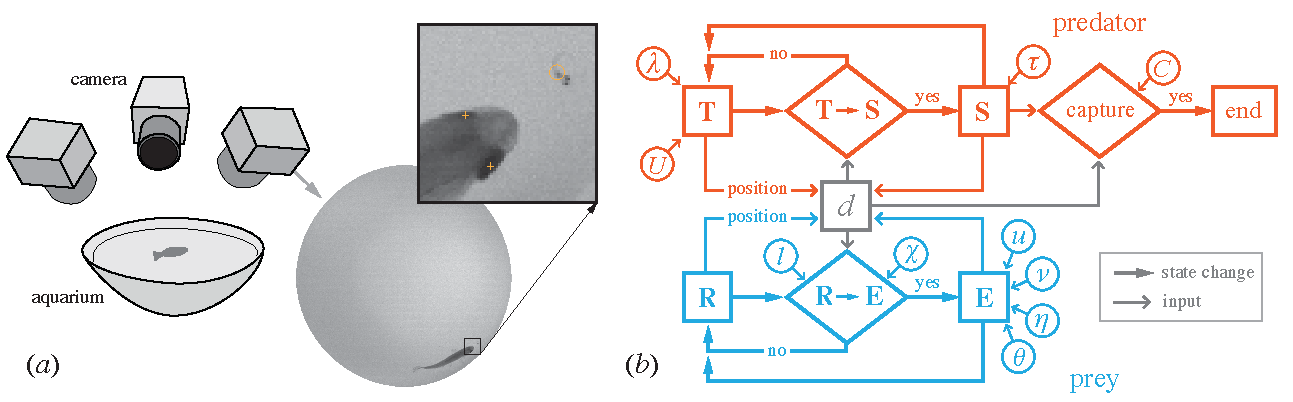
\includegraphics[width=5.5in]{fig_setup}
\caption{Experimental and mathematical techniques for studying predator-prey interactions. 
(\textit{a}) Three high-speed video cameras recorded video of one larval prey and one adult predator fish that were placed in a hemispherical aquarium. 
A representative video frame (cropped to the margin of the aquarium) shows an adult in close proximity to the prey. 
In the inset, white triangles denote the locations of morphological landmarks used to describe the position of the two fish.
 (\textit{b}) A flow chart illustrates the major components of the game model used to simulate the interactions between predators and prey (see Table \ref{table} for symbol definitions and parameter values).}
\label{fig_setup}
\end{figure}

\pagebreak

\begin{figure}[!h]
\centering
	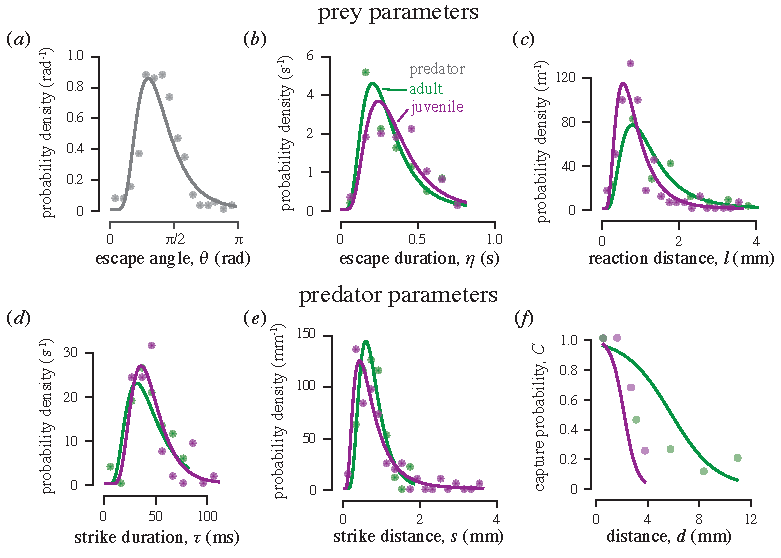
\includegraphics[width=5.5in]{fig_PDFs}
\caption{Descriptive statistics of swimming kinematics. 
(\textit{a-e}) The probability density measurements (circles) and function (Eqn. \ref{eqn_lognorm}) fit for experiments where the predator was a juvenile (purple) or adult (green) predator, which were significantly different, except for escape angle (\textit{a}), shown in gray. 
Parameters were measured from the kinematics of prey (\textit{a-c}) and predators (\textit{d-e}).
(\textit{f}) The capture probability was examined as it varies with distance between the predator and prey (Eqn. \ref{eqn_sig}).  
}
\label{fig_PDF}
\end{figure}

\pagebreak

\pagebreak

\begin{figure}[!h]
\centering
	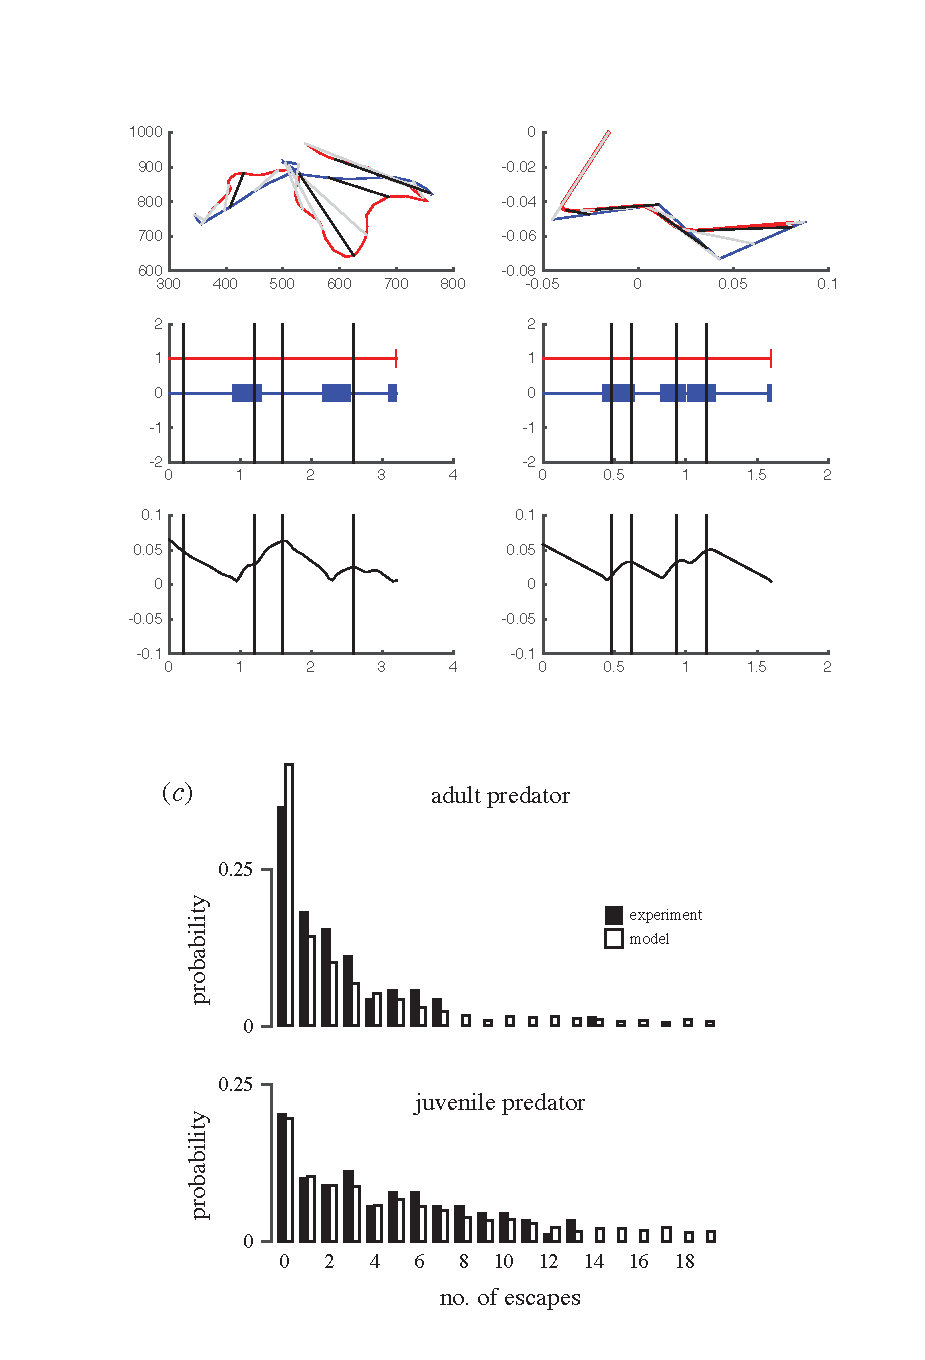
\includegraphics[width=4.5in]{fig_trajectories}
\caption{Comparison between experimental measurements and mathematical modeling. 
(\textit{a}) Trajectories of predator and prey from a representative experiment (left) and simulation (right).
(\textit{b}) Ethograms for these trajectories illustrate the temporal changes in the predator's swimming and strike (left), which are respectively modeled by the T and S (Fig. \ref{fig_setup}\textit{b}) modes (right). 
The prey's behavior while motionless and during escape (left), where modeled with the R and E modes of the model (right).
For both ethograms, the distance between predator and prey are shown and particular moments in the trajectories are highlighted with vertical gray lines.
(\textit{c}) The probability that a prey survives over a particular number of strikes is shown for when the predator was and adult (above) and juvenile (below) for experiments and model simulations.   
}
\label{fig_traj}
\end{figure}

\begin{figure}[!h]
\centering
	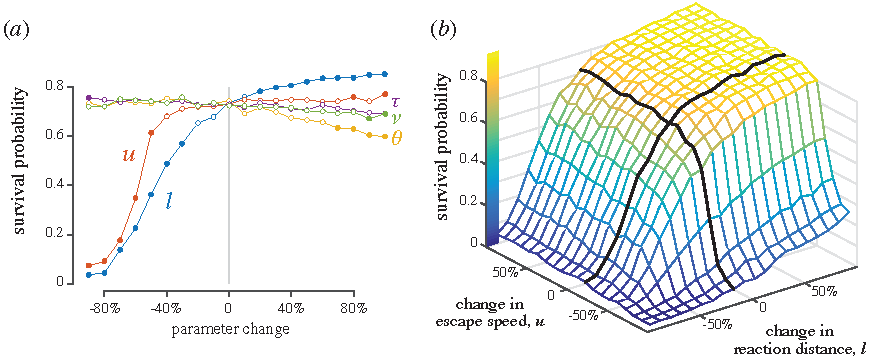
\includegraphics[width=5.5in]{fig_sensitivity}
\caption{Sensitivity analysis of game model to examine the effects of parameter variation on escape probability. 
(\textit{a}) Varying the \hl{log-mean value [MJM:true?]} for the distribution of individual parameters (see Table \ref{table} for parameter definitions and values), with each point representing the result of 1000 simulations. 
(\textit{b}) Variation in escape probability was examined with respect to both escape speed and reaction distance the same simulation results are shown with respect to changes in escape speed (\textit{c}) and reaction distance (\textit{d}).
}
\label{fig_sense}
\end{figure}

\pagebreak



\end{document}